\chapter{Metodologia}

Este capítulo aborda o planejamento e execução do projeto, contendo os procedimentos e técnicas utilizadas, possibilitando a sua  replicação.

Tendo em vista os conceitos descritos nos capítulos anteriores, o presente trabalho tem como objetivo responder à seguinte questão problema:

\begin{center}
\textit{É possível extrair o perfil temático dos deputados através da análise dos seus discursos e proposições utilizando técnicas de aprendizado de máquina e processamento de linguagem natural?}
\end{center}

Além disso, será construído um \textit{website} com o intuito de fornecer uma forma melhor de visualização dos dados obtidos na análise dos discursos e proposições, através de gráficos interativos que garantam que o usuário tenha uma boa experiência ao utilizá-lo.

\section{Trabalhos Relacionados}

Durante a pesquisa bibliográfica realizada neste trabalho, encontrou-se alguns trabalhos que também fizeram análise de textos parlamentares utilizando aprendizado Bayesiano. As seções a seguir descrevem brevemente alguns deles.

\subsection{Retórica Parlamentar}

O Retórica Parlamentar\footnote{http://retorica.labhackercd.net/about.html}, idealizado por Davi Moreira\footnote{https://github.com/davi-moreira}, Manoel Galdino\footnote{https://github.com/mgaldino} e Luís Carli\footnote{https://github.com/luiscarli}, utiliza os discursos proferidos pelos parlamentares no Pequeno Expediente e no Grande Expediente da Câmara dos Deputados para promover a transparência do mandato e fornecer subsídios para o controle social com a divulgação dos temas mais debatidos em Plenário.

A técnica utilizada pelo Retórica para a classificação dos discursos é um modelo Bayesiano hierárquico, descrito por \citeonline{grimmer2009}, onde através de aprendizado não supervisionado são gerados \(k\) \textit{clusters}, sendo \(k\) um valor escolhido ao executar o algoritmo. O resultado é exportado para o formato \textit{csv} e contém os termos mais frequentes de cada cluster. Em seguida, um especialista deve ler e rotular cada \textit{cluster}.

A visualização dos dados é feita através de um gráfico de bolhas, em que cada bolha representa a relevância (medida pela frequência) de cada tema dentre todos os deputados analisados. Dentro de cada bolha são colocados os deputados que enfatizam aquele tema nos seus discursos. Um deputado está associado a um único tema, que é o tema mais enfatizado por ele nos seus discursos.

\begin{figure}[h]
    \centering
    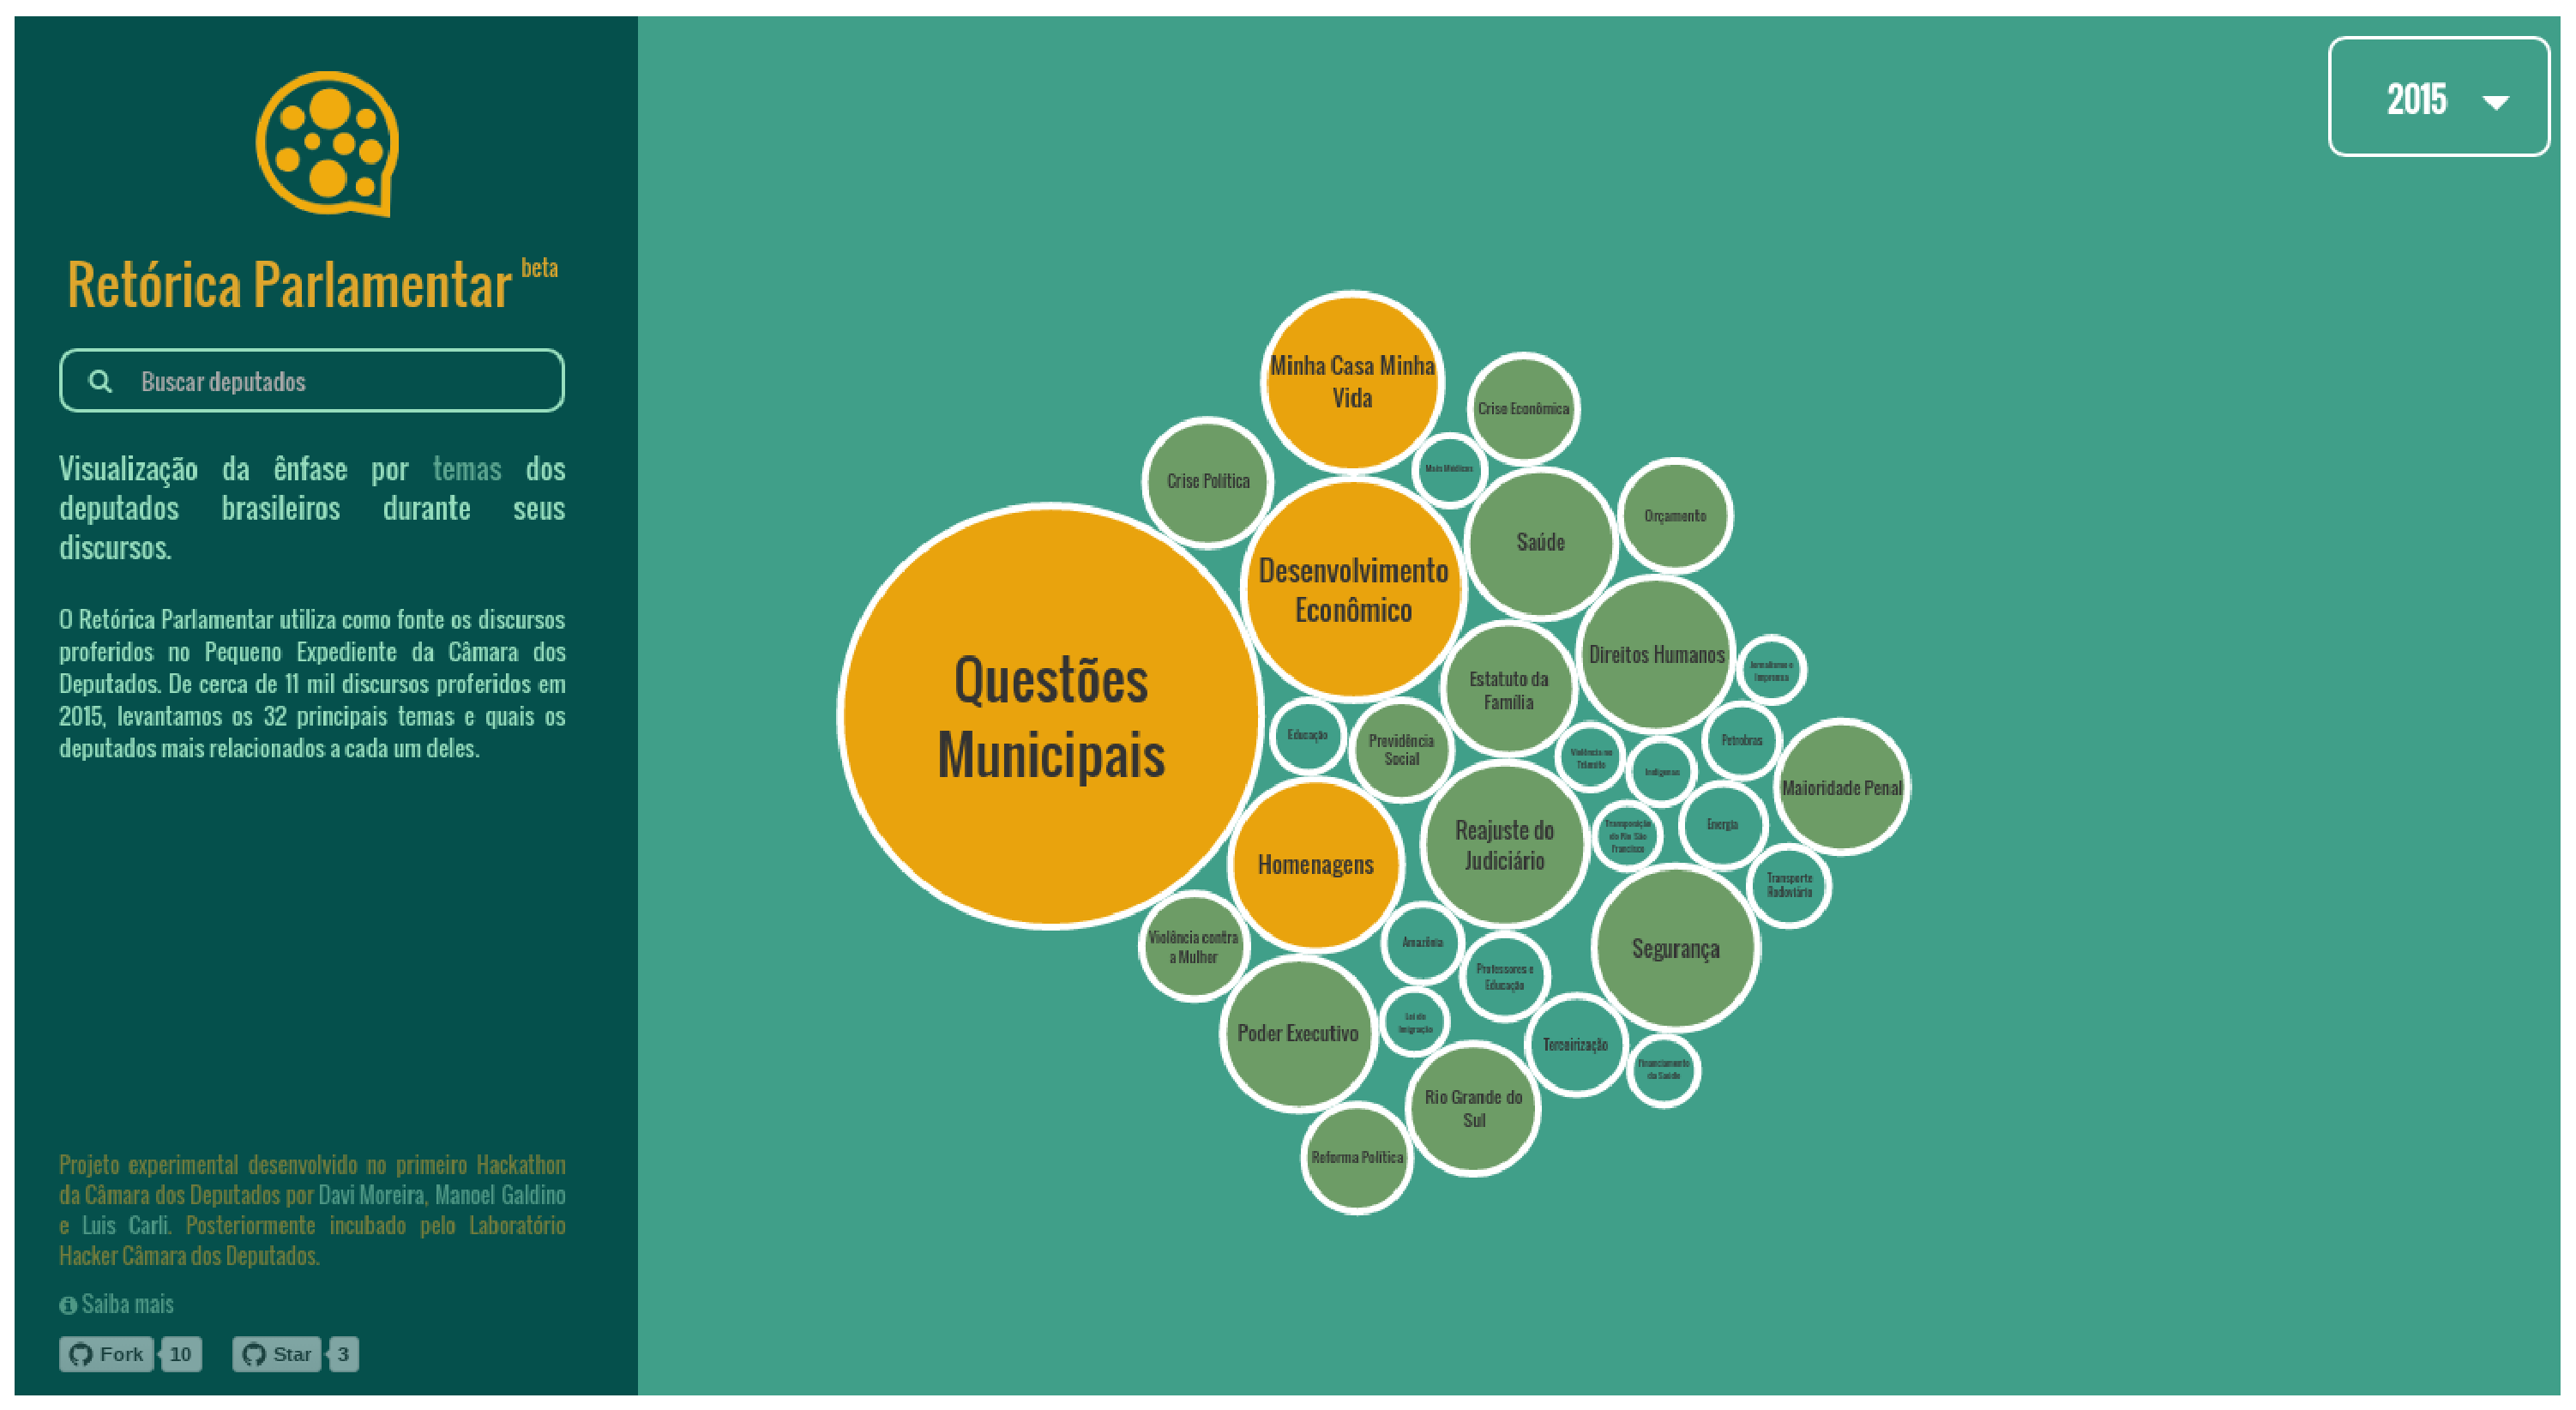
\includegraphics[scale=0.3]{figuras/retorica.eps}
    \caption{Retórica Parlamentar}
\end{figure}


\subsection{\textit{Automatic content analysis of legislative documents by text mining techniques}}

Outro trabalho encontrado foi o de \citeonline{lin}, onde propõem uma análise automática dos dados do parlamento de Taiwan, como questionamentos legislativos, discursos em conferências, proposições legislativas e proposições provisórias do Legislativo de Yuan (poder legislativo unicameral da República da China), utilizando técnicas de processamento de linguagem natural, com o objetivo de representar o desempenho de cada legislador em determinadas categorias, definidas por especialistas do \textit{Institute of Political Science} da \textit{National Sun Yat-sen University}.

\citeonline{lin} definem três aspectos para a análise dos dados do parlamento de Taiwan: direção geográfica, público-alvo e tópico. A direção geográfica se refere ao escopo geográfico abrangido pelos registros legislativos e tem 5 direções. O público-alvo refere-se às pessoas mencionadas explicitamente em seus registros, podendo ser 30 opções. O tópico inclui os temas abordados pelos parlamentares, que possuem um total de 29 tópicos. A figura abaixo mostra os três aspectos e seus valores correspondentes:

\clearpage

\begin{figure}[h]
    \centering
    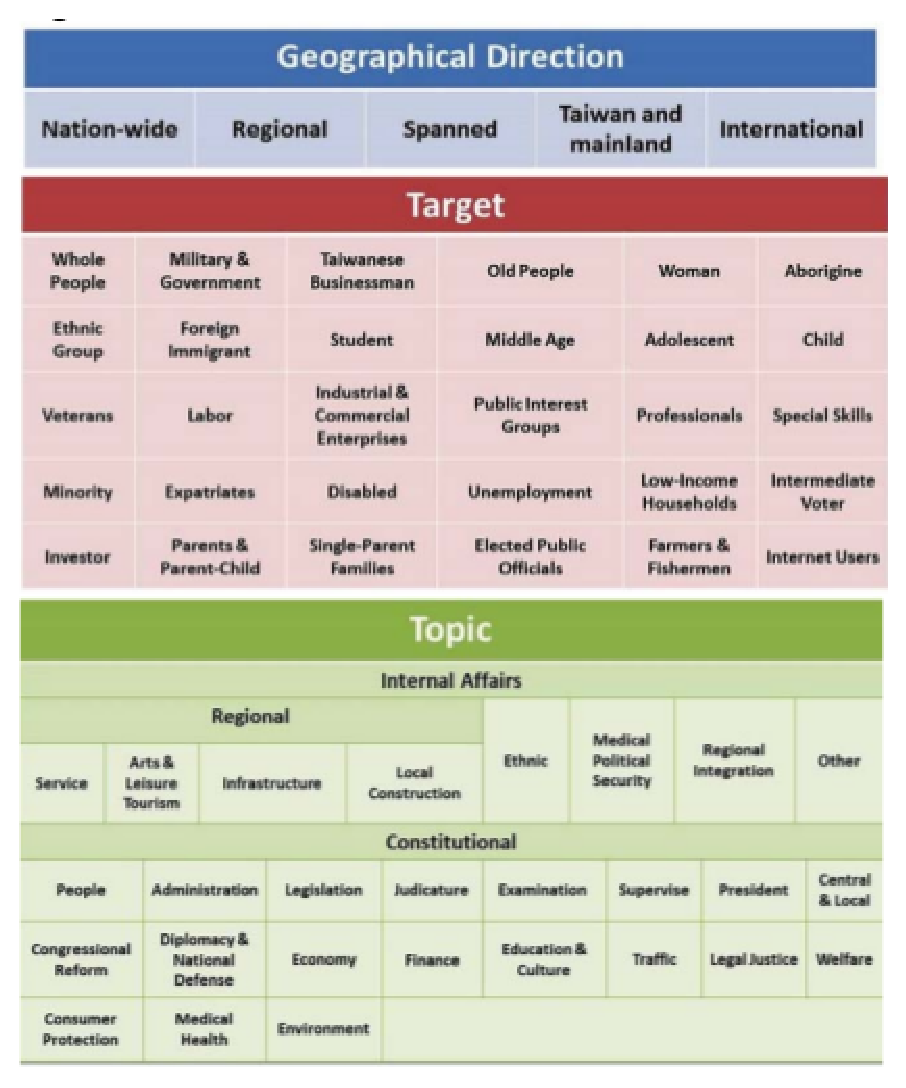
\includegraphics[scale=0.5]{figuras/aspects.eps}
    \caption{Estrutura de categorização}
\end{figure}


Após o processo de pré-processamento do texto, os dados passam por duas fases de clusterização. A primeira fase consiste em uma classificação hierárquica, com o objetivo de obter o número de \textit{clusters} ideal. Em seguida, é aplicado o \textit{k-means}, utilizando o número obtido no processo anterior como valor de \(k\). Dessa forma conseguem melhorar a relevância dos termos que serão apresentados aos especialistas para a definição dos termos que representam as classes.

Os autores disponibilizaram uma interface \textit{web} para os especialistas, para que eles classificassem os quatro tipos de texto (questionamentos legislativos, discursos em conferências, proposições legislativas e proposições provisórias). Esses textos classificados serviram como dados de treinamento e teste do modelo \textit{Support Vector Machine}, adotado para fazer a classificação.

Para representar os dados da análise, foram utilizados gráficos de radar para cada aspecto mencionado anteriormente, como mostram as figuras:

\begin{figure}[h]
  \centering
  \begin{subfigure}{.3\textwidth}
    \centering
    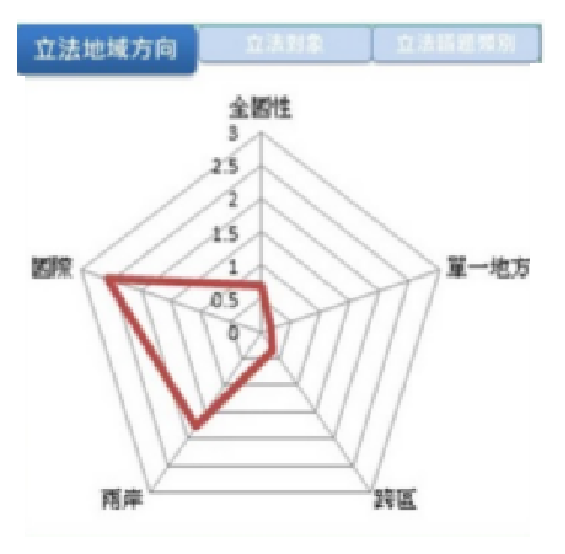
\includegraphics[scale=0.35]{figuras/aspecto1.eps}
  \end{subfigure}%
  \begin{subfigure}{.3\textwidth}
    \centering
    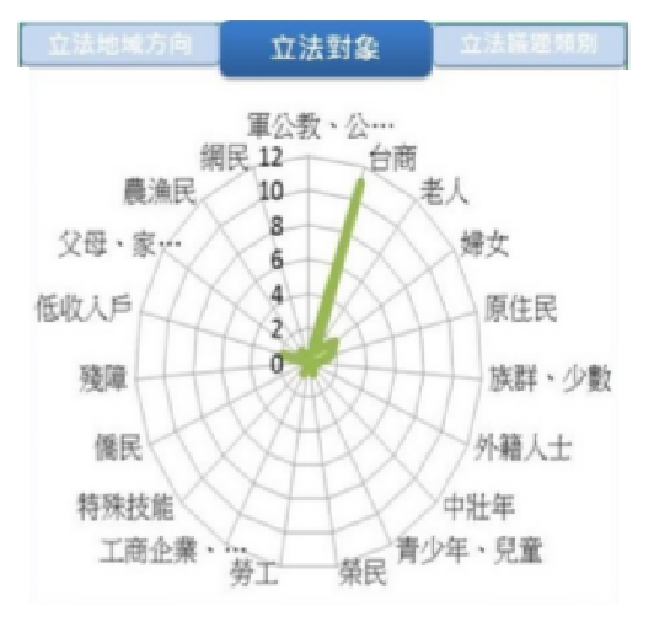
\includegraphics[scale=0.3]{figuras/aspecto2.eps}
  \end{subfigure}
  \begin{subfigure}{.3\textwidth}
    \centering
    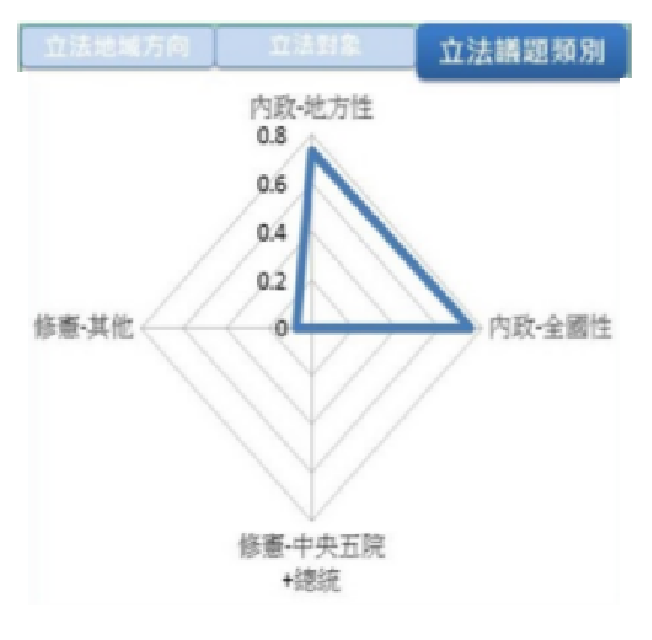
\includegraphics[scale=0.3]{figuras/aspecto3.eps}
  \end{subfigure}
  \caption{Gráficos de desempenho do parlamentar}
\end{figure}

\section{Obtenção dos Dados}
\label{obtencao-dados}

Todos os dados utilizados para análise foram obtidos através do portal de dados abertos da Câmara dos Deputados\footnote{http://www.camara.leg.br/transparencia/dados-abertos}, que é dividido em duas partes: dados legislativos e dados referentes à cota parlamentar, que não foram utilizados nesse trabalho. Os dados legislativos estão relacionados à informações sobre deputados, órgãos legislativos, proposições, sessões plenárias e reuniões de comissões.

\subsection{\textit{Webservice} da Câmara dos Deputados}

Atualmente, o \textit{Webservice} da Câmara dos Deputados é estruturado de acordo com os padrões \textit{SOAP} (\textit{Simple Object Access Protocol}, em português Protocolo Simples de Acesso a Objetos), que se baseiam na linguagem de marcação \textit{XML} e utilizam, principalmente, chamada de procedimento remoto (\textit{RPC}) e protocolo de transferência de hipertexto (\textit{HTTP}) para a transmissão das mensagens \cite{soap2007}.


No entanto, o \textit{webservice} possui alguns aspectos que podem ser melhorados. Como os dados são fornecidos utilizando o formato \textit{XML}, eles não são ``tipados'', ou seja, independente do tipo (inteiro, data, texto, etc) eles são representados com \textit{strings}. Alguns dados são ambíguos, como os referentes aos deputados, onde existem ``ideCadastro'' e ``idParlamentar'', que são utilizados como parâmetros de entrada de requisições distintas. Outro problema é que requisições comuns precisam ser feitas indiretamente pois não agrega conteúdos com \textit{queries} relacionais, como normalmente são as \textit{API REST}. Além disso, o inteiro teor dos discursos parlamentares estão disponíveis apenas em formato \textit{RTF}, o que dificulta um pouco a utilização dos mesmos.

No momento de escrita desse trabalho, a nova \textit{API} de dados abertos ainda se encontra em desenvolvimento e já pode ser acessada pela sociedade\footnote{https://dadosabertos.camara.leg.br/}, porém ainda não possui os mesmos dados disponíveis na versão anterior. Dentre os dados que faltam estão os de discursos em plenário, o que torna o uso dessa nova plataforma desnecessário, já que este é o principal dado utilizado nesse trabalho.

O novo \textit{webservice} segue os padrões REST e possibilita a escolha do formato de retorno, podendo ser em \textit{XML} ou em  \textit{JSON}. Além disso, visa corrigir os problemas encontrados na versão anterior (alguns mencionados nos parágrafos anteriores), bem como aumentar a quantidade de dados disponíveis. Uma das promessas é disponibilizar o texto completo das proposições, que hoje só é disponível via \textit{PDF} sendo que alguns são apenas imagens \textit{scaneadas} dos documentos físicos.

A estrutura do \textit{webservice} da Câmara dos Deputados pode ser encontrada no apêndice \ref{estrutura-webservice}

\subsection{Dados Utilizados}

Para a primeira versão desse trabalho, foram utilizados apenas dados do ano de 2016, tanto para discursos quanto proposições. Foram escolhidos os discursos proferidos no Pequeno Expediente, que é a primeira parte da sessão ordinária do Plenário, tem duração máxima de 60 minutos, é destinado às comunicações de deputados previamente incritos e cada deputado pode discursar por, no máximo, 5 minutos. Já as proposições utilizadas foram apenas Projetos de Lei.

\section{Proposta de Desenvolvimento}

\subsection{\textit{Pygov-br}}

\textit{Pygov-br} é uma biblioteca \textit{python} desenvolvida no contexto desse trabalho cujo objetivo é centralizar o consumo de \textit{APIs} e \textit{webservices} governamentais brasileiros. Além dos dados, a biblioteca também irá fornecer um conjunto de \textit{plugins} para os principais \textit{frameworks} para desenvovimento \textit{web}, para facilitar a utilização dos dados abertos, bem como o cruzamento de dados provenientes de diferentes órgãos governamentais.

Atualmente, a biblioteca oferece suporte somente ao \textit{webservice} da Câmara dos Deputados, tanto para o consumo dos dados quanto para o uso em aplicações \textit{Django}, já que para o desenvolvimento do presente trabalho apenas esses dados seriam utilizados.

A estrutura para o consumo dos \textit{webservices} não é fixa, pois cada \textit{webservice} possui suas características. A implementação para consumir os dados da Câmara dos Deputados segue a estrutura do \textit{webservice} (figura \ref{estrutua_camara_deputados}), com alterações em alguns \textit{endpoints}, conforme mostra a tabela \ref{alteracoes-estrutura-webservice}. Além disso, todos o código implementado foi escrito em inglês, apesar dos dados estarem em português.

\begin{figure}[h]
    \centering
    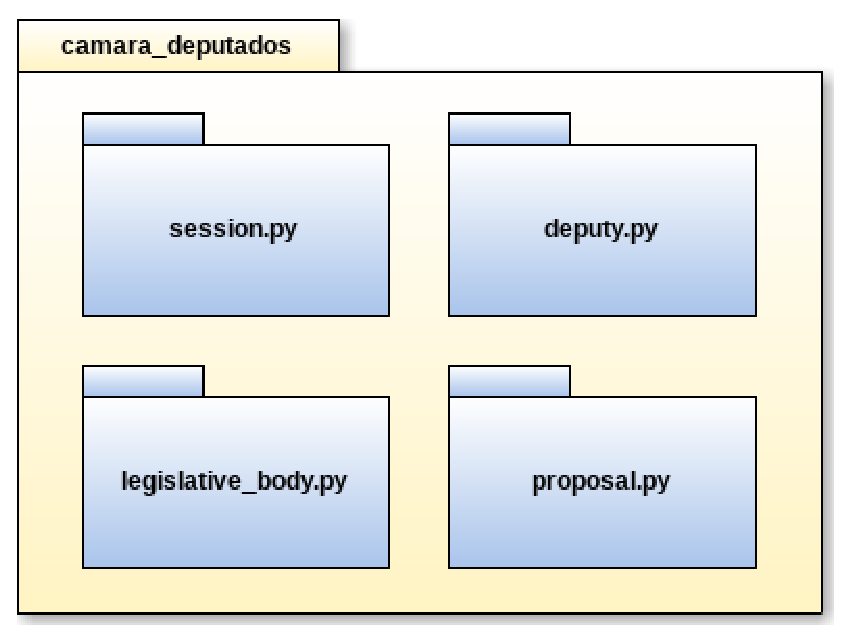
\includegraphics[scale=0.5]{figuras/camara_deputados.eps}
    \caption{Estrutura do módulo de consumo de dados da Câmara dos Deputados}
    \label{estrutua_camara_deputados}
\end{figure}

\begin{table}[h]
\centering
\begin{tabular}{|l|c|c|}
\hline
\multicolumn{1}{|c|}{\textit{\textbf{Endpoint}}} & \multicolumn{1}{c|}{\textbf{Módulo Final}} & \multicolumn{1}{c|}{\textbf{Estrutura do \textit{Webservice}}} \\ \hline
ListarPresencasParlamentar & deputy.py & SessaoReuniao \\ \hline
ObterAndamento & proposal.py & Orgao \\ \hline
ObterEmendasSubstitutivoRedacaoFinal & proposal.py & Orgao \\ \hline
ObterIntegraComissoesRelator & proposal.py & Orgao \\ \hline
\end{tabular}
\caption{Alterações na Estrutura do \textit{Webservice} da Câmara dos Deputados}
\label{alteracoes-estrutura-webservice}
\end{table}

Como dito anteriormente, a \textit{pygov-br} também possui módulos para utilização em conjunto com os \textit{frameworks} de desenvolvimento \textit{web} mais utilizados na comunidade. Porém, como a solução \textit{web} desenvolvida nesse trabalho utilizará o \textit{framework Django}, a atual implementação da \textit{pygov-br} possui suporte somente a esse \textit{framework}.

O módulo \textbf{django\_apps} contém os \textit{plugins} para utilização em projetos \textit{Django}, o que implica na uso da arquitetura \textit{MVT} (\textit{Model View Template}). Similar ao \textit{MVC}, no \textit{MVT} o ciclo começa por uma ação do usuário, a View notifica a Model, para que seu estado seja atualizado, a Model efetua as modificações necessárias e alerta as suas dependências que foi alterada, assim a Template consulta o novo estado da Model, e atualiza a sua visualização.

Entretanto, os \textit{apps Django} da \textit{pygov-br} possuem apenas as \textit{models}, já que o objetivo é somente facilitar a permanência das informações obtidas dos \textit{webservices} governamentais em um banco de dados. No caso da Câmara dos Deputados, os dados utilizados nesse trabalho ficam disponíveis seguindo o modelo entidade-relacionamento na figura \ref{modelo-eer}. Podemos notar que todas as colunas de todas as tabelas se encontram em em inglês, por motivos de padronização do código.


\begin{figure}[h]
    \centering
    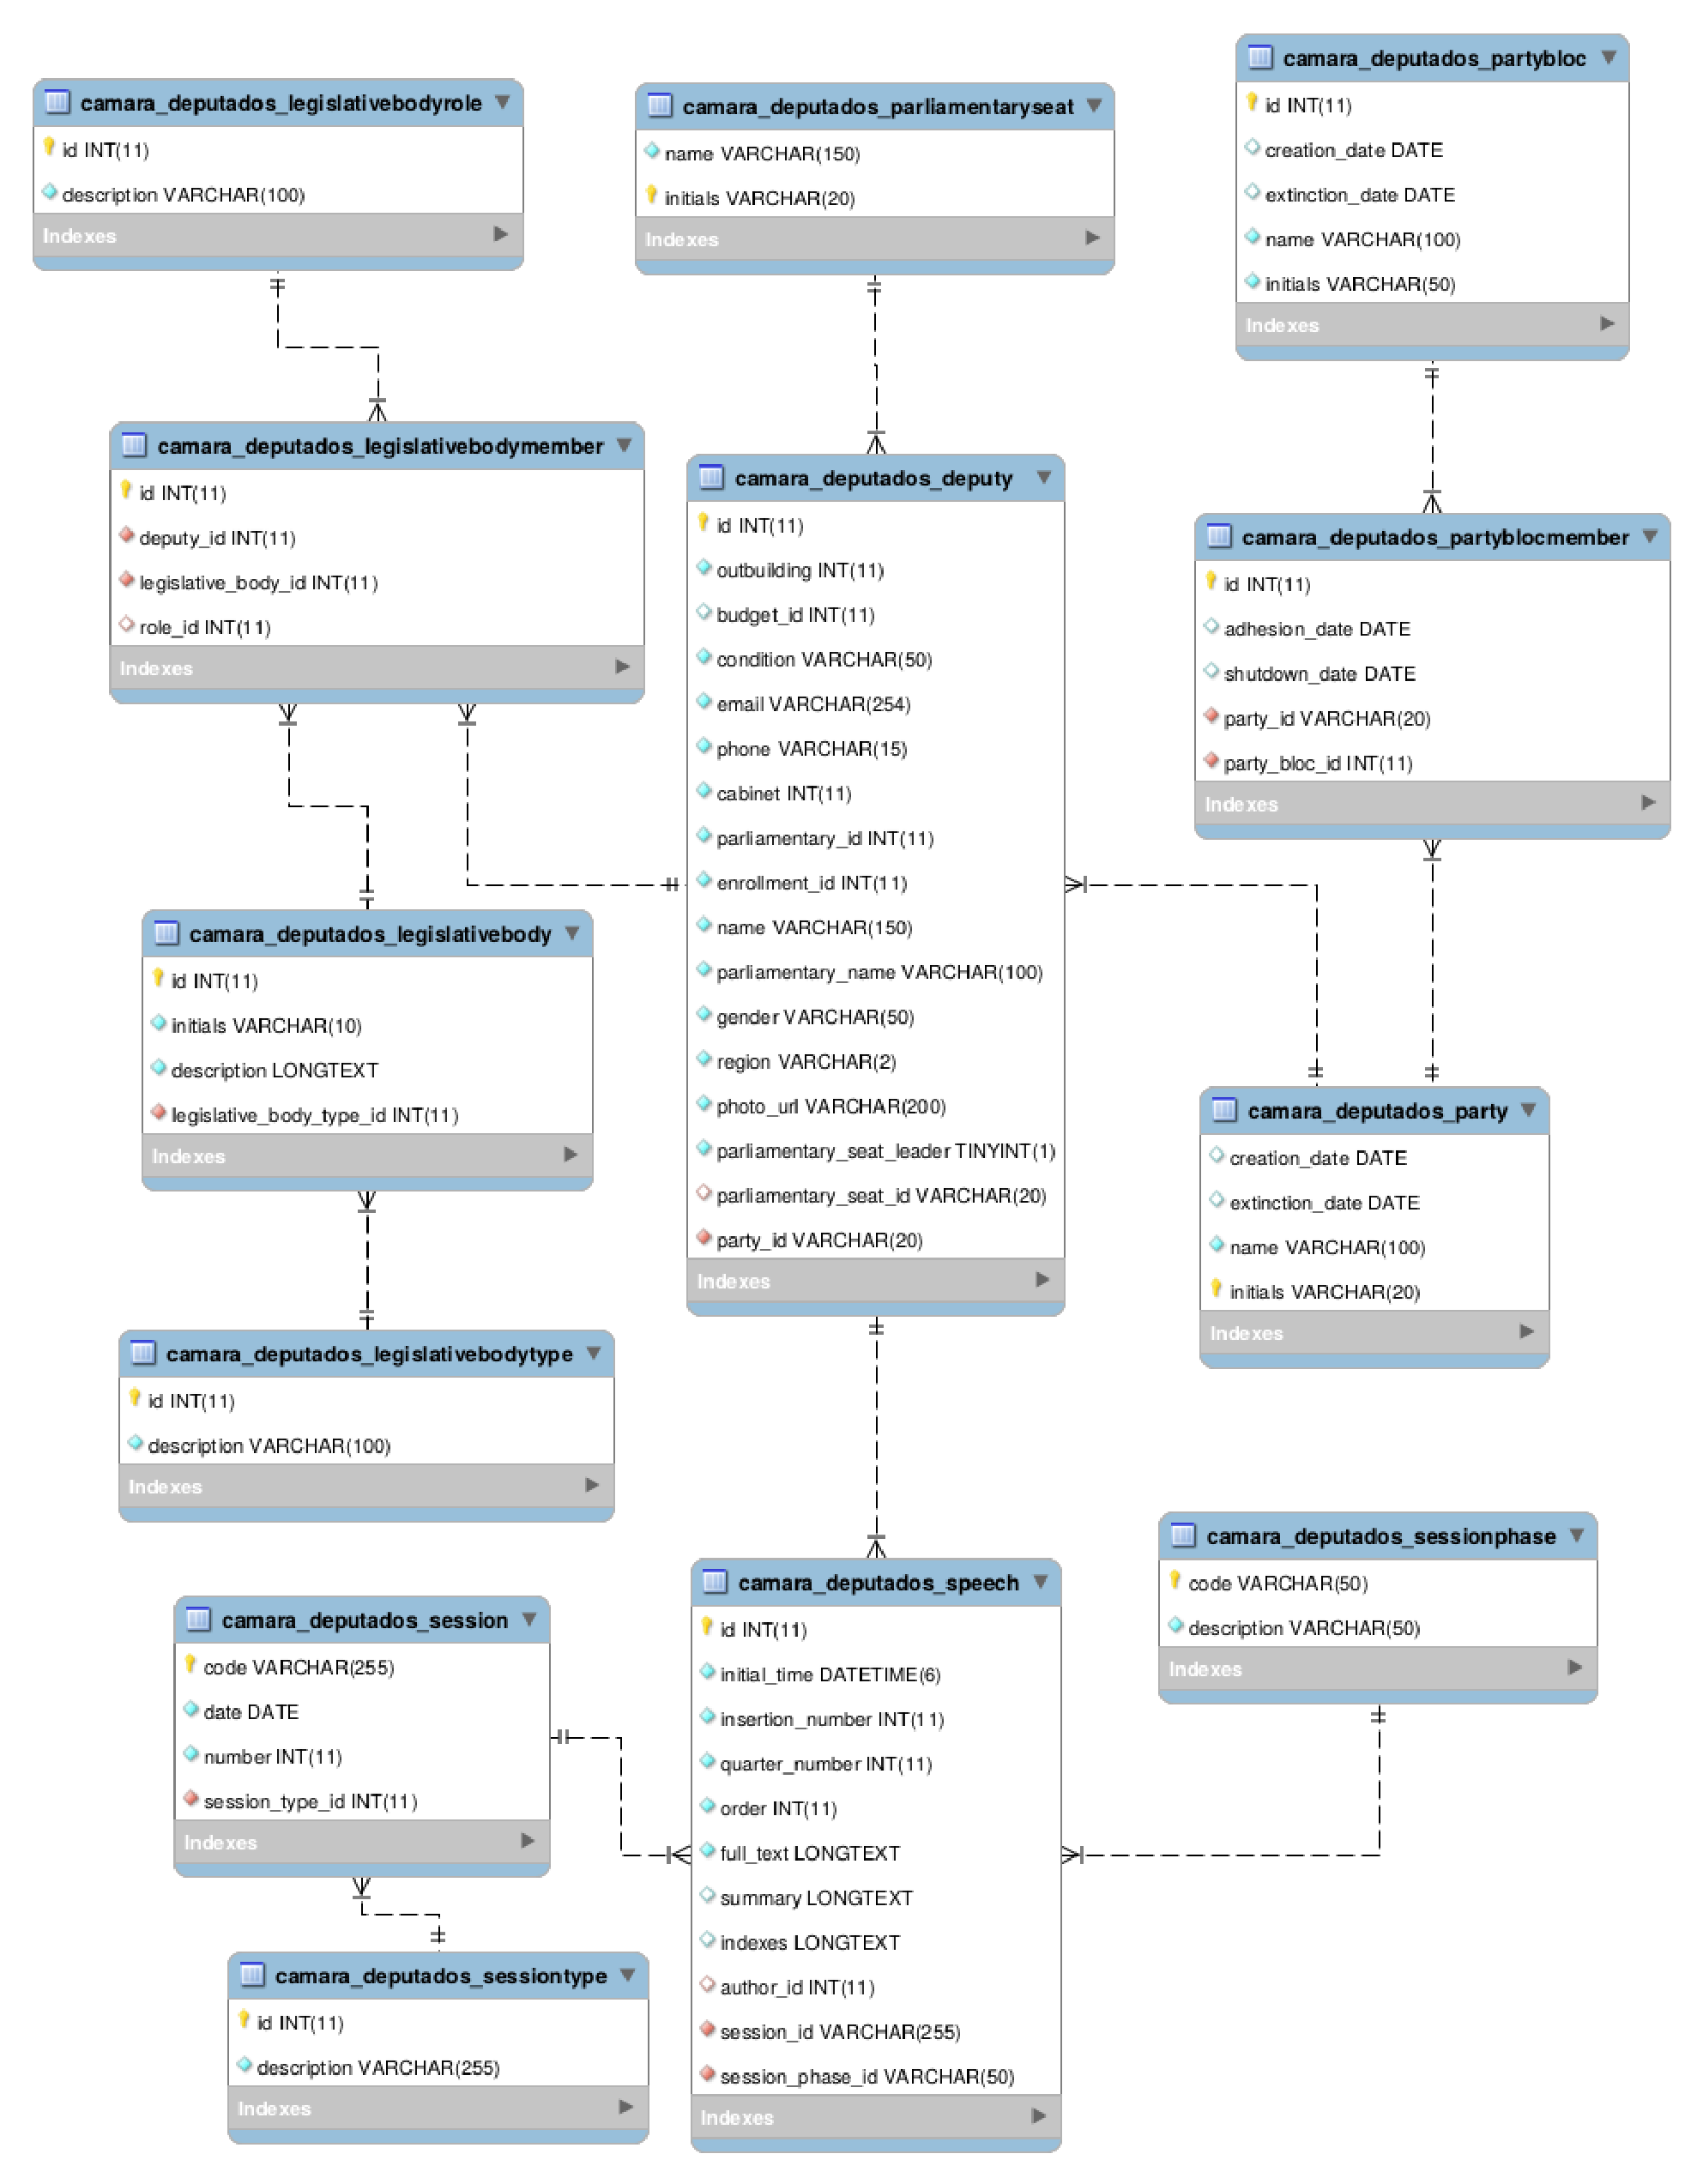
\includegraphics[scale=0.5]{figuras/pygov-eer.eps}
    \caption{Modelo entidade-relacionamento do banco de dados utilizado}
    \label{modelo-eer}
\end{figure}

\clearpage

\subsection{Tenho Dito}

``Tenho Dito'' corresponde ao produto deste trabalho visível pelo usuário final. Trata-se de uma aplicação \textit{web}, desenvolvida utilizando a linguagem \textit{python} com o \textit{framework Django}, e tem como objetivo ser uma forma mais lúdica e amigável de visualização de alguns dados disponíveis nos \textit{webservices} de dados abertos da Câmara dos Deputados. Utiliza métodos de processamento de linguagem natural e aprendizado de máquina para extrair o perfil temático dos parlamentares, analisando o texto de seus discursos e proposições. Além disso, também é possível traçar os temas mais discutidos (tanto em propostas quanto nos próprios discursos) pelos deputados de uma determinada região ou por partidos.

A aplicação é dividida em dois grandes módulos: \textit{nlp} e \textit{application}. O primeiro é responsável por todas as operações relacionadas ao processamento dos textos, o que inclui aprendizado de máquina. Já o segundo módulo é responsável pela parte \textit{web}. No momento de escrita desse trabalho, foi implementado apenas a principal funcionalidade do produto: a análise por estado. E estão disponíveis alguns protótipos de tela, mostrando as possíveis funcionalidades do sistema.

Conforme mencionado no item ``\textit{frameworks}'', em \ref{ferramentas}, a análise dos textos será realizada com o apoio das ferramentas:

\begin{itemize}
    \item \textbf{Plagiarism:} biblioteca em estado \textit{alpha} desenvolvida pelo professor orientador do autor desse trabalho, Fábio Macêdo Mendes, e possui uma série de funcionalidades utilizadas no pré-processamento dos textos, como extração de \textit{tokens}, \textit{stemização}, remoção de \textit{stop words}, geração de \textit{n-gramas} e geração de \textit{bag-of-words} (com os diferentes tipos de representação dos termos, descrito na seção \ref{sec:representação_dos_termos} desse trabalho). Apesar do foco ser a detecção de plágio em textos e códigos, as funcionalidades implementadas podem ser utilizadas em tarefas genéricas de PLN.
    \item \textbf{Textblob:} biblioteca \textit{python} para processamento de dados textuais. Ela fornece uma interface simples para realizar tarefas comuns de processamento de linguagem natural, como análise de sentimento e classificação, por exemplo. Utiliza a biblioteca \textit{NLTK}\footnote{http://www.nltk.org} para realizar essas tarefas.
\end{itemize}

Com o objetivo de deixar registrado as experiências obtidas na primeira parte desse trabalho, dividimos essa seção em duas partes.

\subsubsection{Primeira Parte do Trabalho}

Na primeira parte desse trabalho, a classificação dos discursos e proposições era dividida em duas etapas. A primeira etapa consistia em, inicialmente, dividir o texto em parágrafos, para que a análise fosse realizada com uma quantidade menor de texto, e em seguida os parágrafos seriam classificados entre ``conteúdo útil'' ou ``conteúdo não-útil''. Por exemplo, o trecho \textit{``Muito obrigado, nobre Deputado. Pelo PSOL de São Paulo, o nobre Líder Ivan Valente. V. Exª tem cinco minutos na tribuna.''} não representa um conteúdo significativo, da mesma forma que `\textit{`O SR. ALCEU MOREIRA - Sr. Presidente, primeiro a medida provisória, logicamente.''} também não agregaria nenhum valor à análise. Trechos como esses deveriam ser classificados como ``conteúdo não-útil'' e descartados da análise temática. A segunda etapa do processamento era a classificação temática dos parágrafos classificados como ``conteúdo útil'', na etapa anterior.

Para ambas etapas o procedimento adotado era o mesmo, com algumas alterações nos classificadores. Primeiro, um classificador \textit{NaiveBayesClassifier}, implementado pela biblioteca \textit{textblob}, era instanciado, utilizando dois conjuntos de palavras iniciais, um para definir ``conteúdo não-útil'' e outro para ``conteúdo''. Os conjuntos de palavras podem ser encontrados no apêndice \ref{conjunto-palavras}.

Em seguida, todos os parágrafos eram classificados e, dentre os que foram classificados com uma probabilidade maior que 80\%, os 100 melhores colocados eram utilizados para realizar o treinamento inicial do classificador. A partir disso, era realizado um treinamento supervisionado, onde a aplicação sugeria uma classe mais provável e um especialista humano dizia se o trecho correspondia à classe sugerida, caso não fosse ele deveria fornecer a classe correta. Ao finalizar o treinamento supervisionado, todos os parágrafos eram classificados novamente, agora com o classificador melhor treinado.

Vale observar que as classificações útil/não-útil sugeridas após a primeira fase normalmente correspondiam às corretas, ainda que isto não tenha sido medido explicitamente.

Com o resultado a primeira classificação, obtinha-se um conjunto de parágrafos classificados como ``conteúdo'', que seriam usados na classificação temática. De forma semelhante à primeira classificação, um classificador \textit{NaiveBayesClassifier} era instanciado, agora com um conjunto de palavras específico para cada tema. Os temas e seus respectivos conjuntos de palavras também se encontram no apêndice \ref{conjunto-palavras}.

Todos os parágrafos eram classificados novamente e era gerado um conjunto com os melhores classificados, que era usado para realizar o treinamento inicial do classificador. Após esta etapa, acontecia o treinamento supervisionado, onde um especialista dizia se a classificação sugerida fazia sentido e indicava a classe correta quando não fosse.

Também era possível realizar um treinamento não supervisionado para ambos os classificadores, de forma que as sugestões de classificação eram utilizadas para o treinamento sem a análise de um especialista.

A cada iteração da fase de treinamento todas as probabilidades dos textos adicionados ao classificador são recalculadas, o que implica no aumento significativo do tempo de processamento. Por isso, foi utilizada uma ferramenta de \textit{cache}, possibilitando o armazenamento dos classificadores depois de cada atualização. Toda vez que for realizado um treinamento ou uma classificação seria utilizado o último classificador armazenado em \textit{cache}, com o treinamento prévio.

Esta fase mostrou que alguns discursos são difíceis de classificar ou por terem um conteúdo fragmentado (ex.: parágrafo com apenas uma ou poucas palavras, como \textit{``-Rio de Janeiro''}) ou por conter um conteúdo que aborda mais de um tema simultaneamente (ex.: \textit{``Eu parei de jogar há quase 17 anos e há 15 anos eu criei o Instituto Esporte \& Educação - IEE, do qual sou Presidente, que trabalha com esporte e educação. E há 15 anos nós viajamos para cidades do Brasil que não têm acesso à prática motora na escola, que não têm estrutura, que não têm professores e, especialmente, que não têm a visão da educação física, do esporte, do movimento, da ação motora, da atividade motora como um fator de desenvolvimento, cuja presença é importante dentro da escola.''}).

\subsubsection{Segunda Parte do Trabalho}

Tendo em vista que o resultado das classificações utilizando o modelo descrito acima não foi satisfatório, algumas alterações foram feitas. Tais alterações serão organizadas por tópicos.

\paragraph{Dados Utilizados na Análise}

Em primeiro lugar, passamos a utilizar uma base de palavras pré-classificadas maior: o \textit{thesaurus} da Câmara dos Deputados, que estará deisponível no repositório do Tenho Dito. Esse conjunto de palavras foi utilizado para treinamento do classificador, o que melhorou, mas não o suficiente, o resultado da classificação temática.

Também deixamos de utilizar o texto completo para a análise e passamos a utilizar apenas o sumário, que é basicamente um resumo do discurso/proposição estruturado de forma simples, onde cada sentença corresponde a um tópico abordado pelo deputado (geralmente). Temos, por exemplo, o sumário de um discurso proferido pelo deputado Alberto Fraga, no dia 10/07/2017: \textit{``Incompetência administrativa do Governador Rodrigo Rollemberg. Protesto contra a derrubada de construções na orla do Lago Paranoá, determinada pelo Governo de Brasília. Repúdio à ação ajuizada contra o orador, em face de críticas à administração do Distrito Federal.''}. Analisando o sumário, podemos ver que \textit{``Incompetência administrativa do Governador Rodrigo Rollemberg''} aborda um tema, \textit{``Protesto contra a derrubada de construções na orla do Lago Paranoá, determinada pelo Governo de Brasília''} aborda outro e \textit{``Repúdio à ação ajuizada contra o orador, em face de críticas à administração do Distrito Federal.''} outro. Essa característica permitiu o descarte do primeiro classificador (de ``contúdo útil/não-útil'') e melhorar um pouco a classificação temática, já que as sentenças obtidas trazem um conteúdo relevante, são menores e abrangem menos temas.

Entre os dados de proposições disponíveis no \textit{webservice} de dados abertos da Câmara dos Deputados não encontramos algo semelhante ao sumário dos discursos, apenas a ementa da proposição, mas que na maioria das vezes contém algo muito técnico, sendo necessário o conhecimento mais profundo das leis, como por exemplo: \textit{``Revoga os artigos 165, 166 e 204 do Decreto-Lei nº 1.001, de 21 de outubro de 1969.''}. Buscando utilizar os mesmos dados, tanto para dicursos quanto para proposições, optou-se pela utilização da indexação realizada pela Câmara dos Deputados, já que a mesma está presente em todos os dicursos realizados no Pequeno Expediente e em todos os Projetos de Lei. Somente para exemplificar, o Projeto de Lei que possui a ementa citada anteriormente, possui a seguinte indexação: \textit{``Revogação, dispositivo legal, Decreto-Lei, Código Penal Militar, promoção, reunião, publicação, crítica, indevido, exercício, comércio, militar da ativa''}, o que permite o entendimento do que realmente a proposição aborda.

\paragraph{Modelos Utilizados}

Na primeira parte desse trabalho, tentou-se utilizar uma abordagem não-supervisionada com o \textit{k-means} e ao não obter um resultado satisfatório, optou-se pela utilização do \textit{Naive Bayes}. Este, por sua vez, define apenas uma classe para cada texto analisado, mesmo quando o texto aborda mais de um tema. Com o objetivo de identificar mais de um tema por discurso, iniciou-se o estudo do modelo \textit{LDA}.

O \textit{LDA} é, naturalmente, não-supervisionado. Entretanto, a implementação da biblioteca \textit{Gensim}\footnote{\lnk{Gensim}{https://radimrehurek.com/gensim/models/ldamodel.html\#gensim.models.ldamodel.LdaModel}} permite inserir informações a priori no algoritmo.

Para aplicar o \textit{LDA}, instanciamos um objeto da classe \textit{LdaModel} passando como parâmetros o \textit{corpus} de treinamento utilizado (\textit{thesaurus}), a quantidade de tópicos a serem encontrados e o \textit{eta}, que será utilizado pelo algoritmo para definir probabilidades a priori. O \textit{eta} é uma matriz \(K \times n\), onde \(K\) é o número de tópicos e \(n\) o número de termos. Com essa matriz, podemos definir valores específicos para determinadas palavras em relação aos tópicos, sendo que o valor padrão para cada palavra é de \(\frac{1}{K}\). Dessa forma, os termos já classificados pelo \textit{thesaurus} foram inseridos no \textit{LDA} através do \textit{eta}, onde a valor dos termos em seus tópicos passam ser definidos de acordo com a seguinte equação:
\begin{align}
  \frac{1}{K}+\frac{(K-1)}{K} \cdot F,
\end{align}
onde \(K\) é a quantidade de tópicos e \(F\) é \(0.99^6\). O valor de \(F\) foi escolhido para ser o menor número que classifica todos os conhecidos corretamente, e a ideia do expoente foi somente para ajustar esse peso. Dessa forma, o \textit{training set} é classificado corretamente e o tópico correto sempre com mais de 50\%.

Para visualizar os dados obtidos com o \textit{LDA}, utilizamos o método \textit{PCA} (\textit{Principal Component Analysis}), que tenta capturar as componentes principais de um conjunto de dados e projeta em um espaço de dimensão mais baixa, para mostrar os dados em duas dimensões. O \textit{LDA} funciona bem quando o \textit{PCA} consegue dividir o \textit{dataset} em \textit{clusters} relativamente bem definidos. No gráfico abaixo, os pontos marcados correspondem a um \textit{cluster} conhecido específico.

\begin{figure}[h]
    \centering
    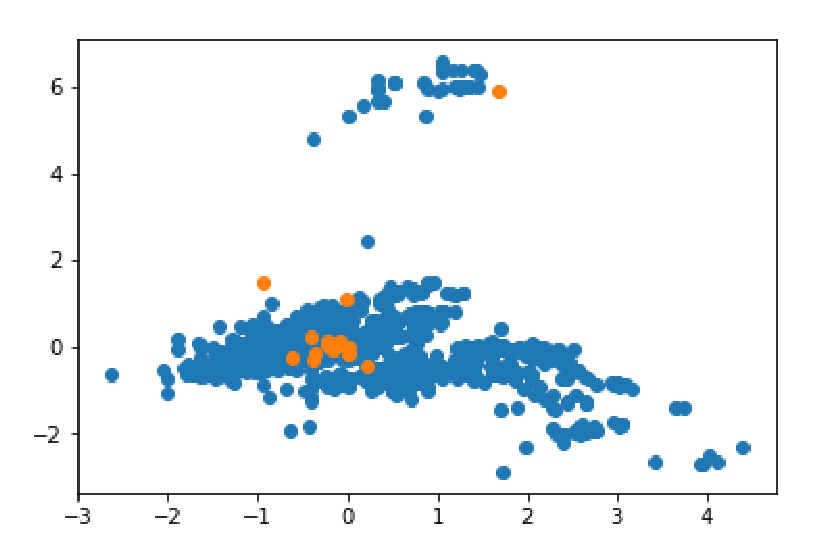
\includegraphics[scale=0.5]{figuras/pca.eps}
    \caption{Análise dos dados do \textit{LDA} utilizando \textit{PCA}}
\end{figure}

Os \textit{clusters} podem estar em mais de duas dimensões, porém analisando os nossos dados, mesmo em duas dimensões, conseguimos visualizar  apenas um \textit{cluster} separado e todo o resto junto, mostrando que a classificação claramente não está correta.

Tendo em vista o resultado acima, voltamos a utilizar o modelo \textit{naive Bayes} para realizar a classificação dos discursos e proposições.

\paragraph{Classificação dos Discursos e Proposições}

Como dito nos tópicos anteriores, serão utilizados os dados do \textit{thesaurus} da Câmara dos Deputados para o treinamento, a indexação dos discursos e proposições para e o classificador \textit{naive Bayes} para a análise.

Primeiramente, assim como na primeira parte do trabalho, é instanciado um objeto da classe \textit{NaiveBayesClassifier}, implementado pela biblioteca \textit{textblob}, passando como treinamento inicial o conjunto de termos já classificados do \textit{thesaurus}. Com o classificador treinado, passamos por cada discurso e em cada um deles obtemos a lista de termos usados em sua indexação. Cada termo é analisado individualmente e apenas aqueles que forem classificados com a probabilidade maior que 60\% são utilizados, o restante é descartado. Após classificar todos os termos de indexação de um discurso, calculamos a porcentagem de cada tema e atribuímos ao discurso. Por exemplo, suponha um discurso possui 13 termos na indexação e apenas 8 deles foram classificados com probabilidade maior que 60\%. Se 4 desses foram classificados como ``Segurança'', 3 como ``Direitos Humanos'' e 1 como ``Saúde'', então o discurso será classificado como sendo 50\% sobre segurança, 37,5\% direitos humanos e 12,5\% saúde. Além disso, definimos como tema principal do discurso aquele com maior porcentagem.

Vale enfatizar que as porcentagens mostradas pelo \textit{naive Bayes} são interpretadas de forma diferente que o \textit{LDA}. Enquanto no segundo trata-se de uma mistura de temas, no \textit{naive Bayes} correspondem à chance de um texto pertencer exclusivamente a cada tópico.

Para as proposições, os mesmos procedimentos são realizados, bem como a utilização do mesmo classificador já treinado.

\paragraph{Classificação dos Deputados}

Uma vez que todos os discursos e proposições estejam classificados, passamos por todos os deputados e em cada um deles obtemos uma lista de discuros e uma lista de proposições. Somamos todas as porcentagens, de todos os temas de discursos e proposições e dividimos pela soma da quantidade de discursos e proposições. Por exemplo, suponha que um parlamentar possui dois discursos e uma proposição classificada. Seu primeiro discurso é 100\% sobre ``Direitos Humanos'' e o segundo 70\% ``Saúde'' e 30\% ``Direitos Humanos''. A proposição foi classificada como 60\% ``Segurança'' e 40\% ``Educação''. Temos então que a classificação final do deputado seria: 43,3\% ``Direitos Humanos'', 23,3\% ``Saúde'', 20\% ``Segurança'' e 13,3\% ``Educação''. Assim como nos discursos e proposições, o tema com maior porcentagem é o tema principal de um deputado.

\paragraph{Classificação dos Estados}

Após a classificação dos deputados, passamos por todos os estados e em cada um obtemos a lista de parlamentares que o representam. Utilizando o mesmo procedimento da classificação dos deputados, somamos todas as porcentagens temáticas dos deputados e dividimos pela quantidade total de deputados.

\paragraph{Acurácia}

Após a mudança dos dados utilizados na análise, pudemos notar uma melhoria significativa no resultado da classificação. Utilizando como treinamento 11.151 termos, presentes no \textit{thesaurus}, e como teste 111 novos termos, obtidos da indexação dos próprios discursos e proposições, classificados manualmente pelo autor, obtivemos um índice de acerto de 59,46\%. Justificando, assim, a escolha de classificações apenas com probabilidade maior que 60\%, descrito nos itens anteriores.


